\documentclass[12pt]{article}
\usepackage{graphicx,import}
\usepackage{float}
\usepackage[svgnames]{xcolor} 
\usepackage{makecell}
\usepackage{fancyhdr}
\usepackage{subcaption}
\usepackage{hyperref}
\usepackage{enumitem}
\usepackage[many]{tcolorbox}
\usepackage{listings }
\usepackage[a4paper, total={6in, 8in} , bottom = 25mm , top = 25mm, headheight = 1.25cm , includehead,includefoot,heightrounded ]{geometry}
\usepackage{afterpage}
\usepackage{amssymb}
\usepackage{pdflscape}
\usepackage{gensymb}
\usepackage{textcomp}
\usepackage{tikz,pgfplots}
\usepackage{xecolor}
\usepackage{rotating}
\usepackage{pdfpages}
\usepackage[Kashida]{xepersian}
\usepackage[T1]{fontenc}
\usepackage{tikz}
\usepackage[utf8]{inputenc}
\usepackage{PTSerif} 
\usepackage{seqsplit}
\usepackage{hhline}
\usepackage{pgfgantt}
\usepackage{graphicx}
\usepackage{filecontents}
\usepackage{url} % for "\url" macro
\usepackage{babel}
\usepackage[backend=bibtex, style=numeric]{biblatex}

\addbibresource{refs.bib}

\graphicspath{ {./images/} }

\renewcommand\theadalign{bc}
\renewcommand\theadfont{\bfseries}
\renewcommand\theadgape{\Gape[4pt]}
\renewcommand\cellgape{\Gape[4pt]}

\usepackage[edges]{forest}

\usepackage{listings}
\usepackage{xcolor}

\hypersetup{
	colorlinks   = true, %Colours links instead of ugly boxes
	urlcolor     = blue, %Colour for external hyperlinks
	linkcolor    = blue, %Colour of internal links
	citecolor   = red %Colour of citations
}
 
\definecolor{codegreen}{rgb}{0,0.6,0}
\definecolor{codegray}{rgb}{0.5,0.5,0.5}
\definecolor{codepurple}{rgb}{0.58,0,0.82}
\definecolor{backcolour}{rgb}{0.95,0.95,0.92}
 
\NewDocumentCommand{\codeword}{v}{
\texttt{\textcolor{blue}{#1}}
}
\lstset{language=java,keywordstyle={\bfseries \color{blue}}}


\lstdefinestyle{mystyle}{
    backgroundcolor=\color{backcolour},   
    commentstyle=\color{codegreen},
    keywordstyle=\color{magenta},
    numberstyle=\tiny\color{codegray},
    stringstyle=\color{codepurple},
    basicstyle=\ttfamily\normalsize,
    breakatwhitespace=false,         
    breaklines=true,                 
    captionpos=b,                    
    keepspaces=true,                 
    numbers=left,                    
    numbersep=5pt,                  
    showspaces=false,                
    showstringspaces=false,
    showtabs=false,                  
    tabsize=2
}

\lstset{style=mystyle}

\settextfont[Scale=1.2, Path = fonts/ ,BoldFont={Bahij Nazanin-Bold} , ItalicFont = {IRNazaninIranic}]{Bahij Nazanin-Regular}
% \setlatintextfont[Scale = 1.0, Path = fonts/]{Garamond}
% \DefaultMathsDigits 
\DeclareMathSizes{11}{19}{13}{9} 
%\DeclareMathSizes{12}{14.4}{8}{9}





\newenvironment{changemargin}[2]{%
\begin{list}{}{%
\setlength{\topsep}{0pt}%
\setlength{\leftmargin}{#1}%
\setlength{\rightmargin}{#2}%
\setlength{\listparindent}{\parindent}%
\setlength{\itemindent}{\parindent}%
\setlength{\parsep}{\parskip}%
}%
\item[]}{\end{list}}


\definecolor{foldercolor}{RGB}{124,166,198}

\tikzset{pics/folder/.style={code={%
    \node[inner sep=0pt, minimum size=#1](-foldericon){};
    \node[folder style, inner sep=0pt, minimum width=0.3*#1, minimum height=0.6*#1, above right, xshift=0.05*#1] at (-foldericon.west){};
    \node[folder style, inner sep=0pt, minimum size=#1] at (-foldericon.center){};}
    },
    pics/folder/.default={20pt},
    folder style/.style={draw=foldercolor!80!black,top color=foldercolor!40,bottom color=foldercolor}
}

\forestset{is file/.style={edge path'/.expanded={%
        ([xshift=\forestregister{folder indent}]!u.parent anchor) |- (.child anchor)},
        inner sep=1pt},
    this folder size/.style={edge path'/.expanded={%
        ([xshift=\forestregister{folder indent}]!u.parent anchor) |- (.child anchor) pic[solid]{folder=#1}}, inner xsep=0.6*#1},
    folder tree indent/.style={before computing xy={l=#1}},
    folder icons/.style={folder, this folder size=#1, folder tree indent=3*#1},
    folder icons/.default={12pt},
}

\begin{document}


%%% title pages
\begin{titlepage}
\begin{center}
        
\vspace*{0.7cm}


\includegraphics[width=0.4\textwidth]{sharif1.png}\\
\vspace{0.5cm}
\textbf{ \Huge{\emph ‌آزمایشگاه سخت‌افزار} }\\
\vspace{0.5cm}
\textbf{ \Large{گزارش فاز دوم} }
\vspace{0.2cm}
       
 
      \large \textbf{دانشکده مهندسی کامپیوتر}\\\vspace{0.2cm}
    \large   دانشگاه صنعتی شریف\\\vspace{0.2cm}
       \large   ﻧﯿﻢ سال اول 02-01 \\\vspace{0.2cm}
      \noindent\rule[1ex]{\linewidth}{1pt}
استاد:\\
    \textbf{{جناب آقای دکتر اجلالی}}


دستیار آموزشی:\\
\textbf{{جناب آقای دکتر فصحتی}}

    \vspace{0.25cm}
    
    موضوع پروژه:\\
    
    \textbf{دید در شب اتومبیل}
    
    \vspace{0.35cm}
    
    
        شماره گروه:
    \textbf{{۶}}\\
    
اعضای گروه:\\

    \textbf{{علیرضا شاطری}}
    \\
   
     \textbf{{رضا امینی}}   
\end{center}
\end{titlepage}
%%% title pages


%%% header of pages
\newpage
\pagestyle{fancy}
\fancyhf{}
\fancyfoot{}
\cfoot{\thepage}
\chead{}
\rhead{
\includegraphics[width=0.1\textwidth]{sharif.png}}
\lhead{گزارش فاز دوم}
%%% header of pages

\newfontfamily\terminal{Courier New Bold}

\KashidaOff
 \newcommand{\inlineLatin}[1]{
	\small{\lr{{\terminal #1}}}
}


\tableofcontents
\listoffigures
\listoftables

\newpage
\section{مقدمه}

محصول نهایی این پروژه، یک سیستم دید در شب است که درون اتومبیل قرار می‌گیرد و به راننده هنگام رانندگی در تاریکی، کمک به سزایی می‌کند. در این سیستم اطلاعات از طریق یک دوربین حرارتی به ماژول رزپری منتقل می‌شود و کدهایی که در رزپبری قرار داده شده است با انجام پردازش تصویری ساده، تشخیص خواهد داد که آیا موجود زنده‌ای در میدان دید راننده حضور دارد یا خیر. همچنین از طریق چراغ و صدا نتیجه را به راننده اطلاع می‌دهد.
\\

ما در این فاز قصد داریم تا تصمیم نهایی برای استفاده از ماژول ها داشته باشیم، و همچنین برای چراغ های اخطار پیاده سازی کد را انجام دهیم و آن را به طور کامل تست کنیم. 

\section{گزارش انجام پروژه}
\subsection{تصمیم نهایی}

با توجه به گزارش فاز اول ما برای استفاده از دوربین حرارتی و دوربین دید در شب مزایا و معایبی بیان کردیم، اما دو پارامتر برای ما مهمتر از بقیه ی موارد بود، اول اینکه یک ماژول برای کار ما کاربردی باشد و حتما پاسخ‌گو سوال های ما باشد، و مورد دوم اینکه کد های آماده وجود داشته باشد، زیرا پروژه برای درس آزمایشگاه سخت افزار می‌باشد و خواسته ی پروژه بیشتر باید سخت افزاری و کار با سخت افزار باشد.
\\
برای دوربین دید در شب ما نیاز به پیاده سازی یک مدل یادگیری ماشین داریم که با جستجو هایی که انجام دادیم متاسفانه نتوانستیم کد آماده ای پیدا کنیم در نتیجه انتخاب این ماژول برای ما سخت شد، اما مطمئن هستیم که دوربین دید در شب پاسخ‌گو خواهد بود، همچنین برای دوربین حرارتی ما توانستیم منابع زیادی پیدا کنیم  . با توجه به اینکه کد های زیادی در مورد یافتن انسان با استفاده از این ماژول وجود داشت، پس تصمیم نهایی ما بر این شد که دوربین حرارتی را انتخاب کنیم.

\newpage
\subsection{اتصال چراغ های اخطار}

\subsubsection{اتصال فیزیکی}

در قسمت اول کار ما باید چراغ ها را به رزپبری پای متصل میکردیم که این کار به سادگی انجام شد.

\begin{figure}[h]
	\begin{center}
		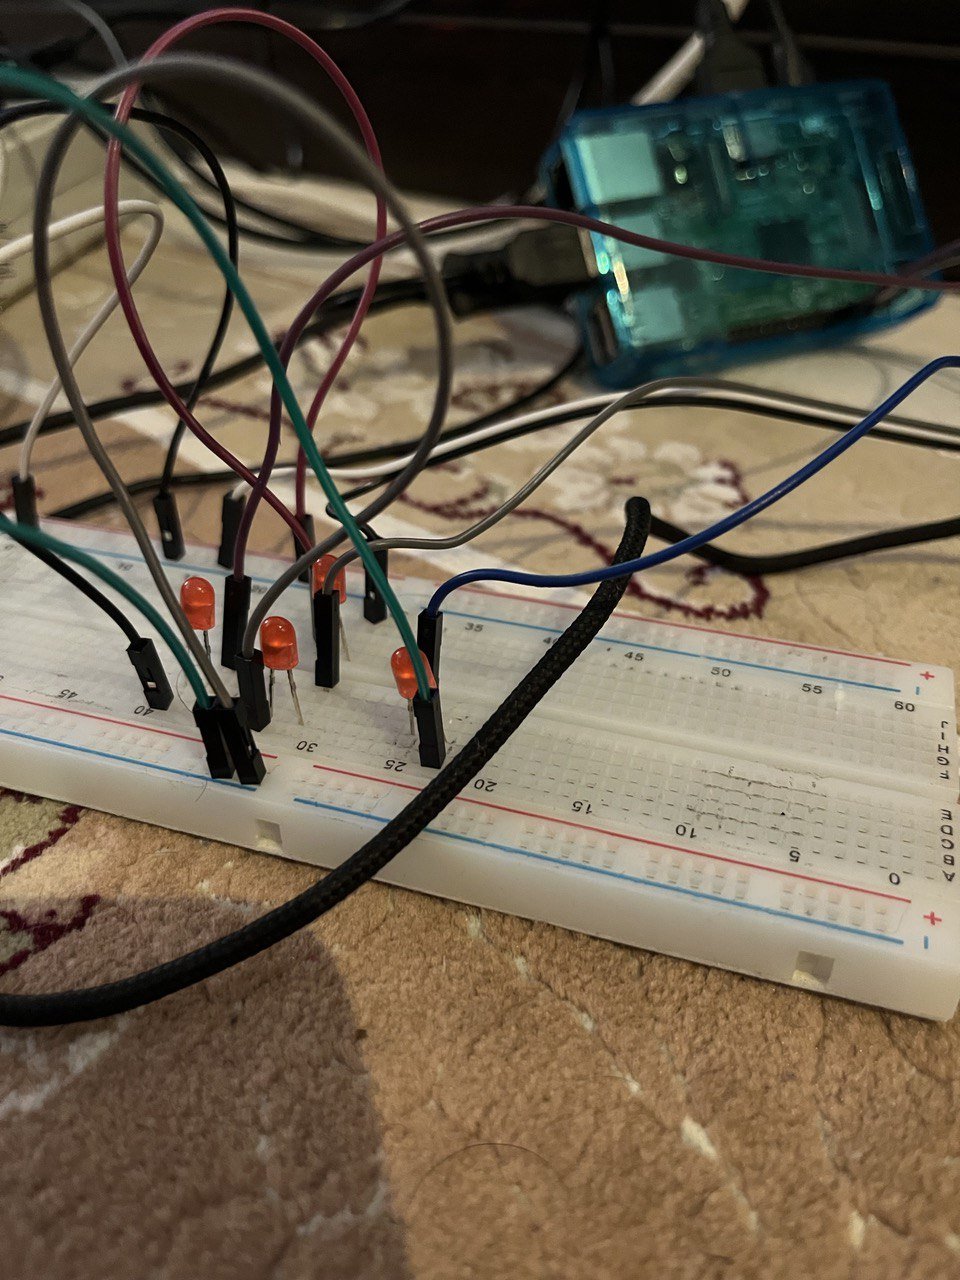
\includegraphics[width=.50\textwidth]{images/led.jpg}
	\end{center}
	\caption{اتصال چراغ}
\end{figure}

\subsubsection{پیاده سازی کد}


در مرحله بعد ما یک کد یکپارچه آماده کردیم که با صدا کردن دو تابع یک چراغ خاص را میتوان خاموش و یا روشن کرد.

\\ 

\begin{figure}[h]
	\begin{center}
		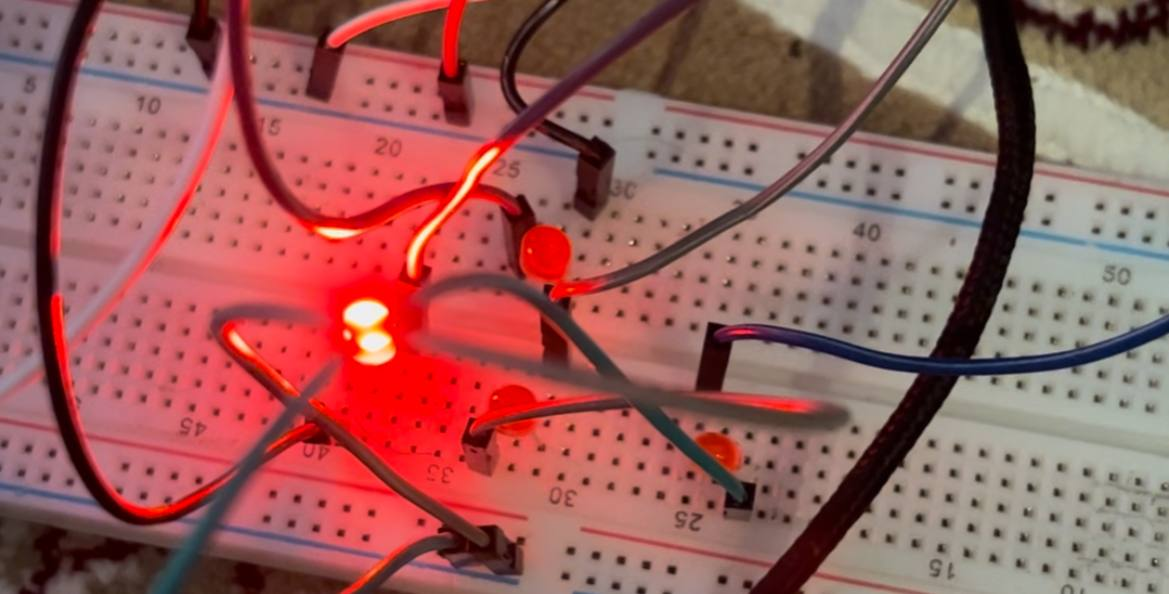
\includegraphics[width=.50\textwidth]{images/led-on.jpg}
	\end{center}
	\caption{چراغ روشن}
\end{figure}
\\

\newpage

\subsection{اتصال سنسور دما}

\subsubsection{اتصال فیزیکی}

حالا نوبت اتصال ماژول اصلی پروژه است، سنسور دما را با استفاده از راهنمای زیر به رزپبری پای نصب کردیم.

\begin{figure}[h]
	\begin{center}
		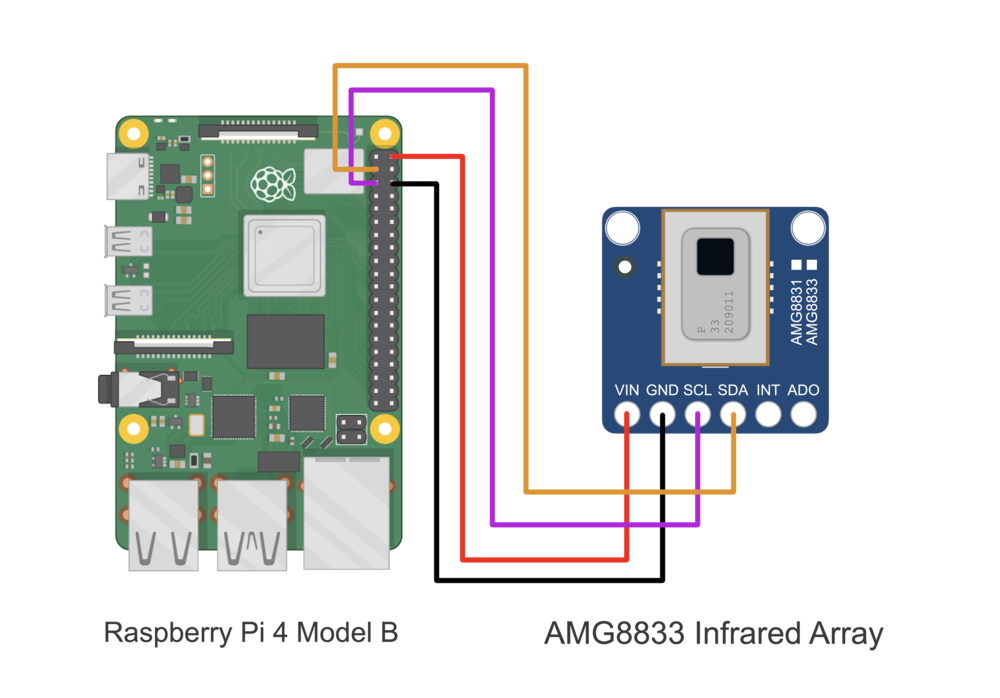
\includegraphics[width=.75\textwidth]{images/amg8833_RPi4_wiring.png}
	\end{center}
	\caption{راهنمای نصب سنسور دما}
\end{figure}

\subsubsection{پیاده سازی کد}

در این فاز ما موفق به پیاده سازی کد برای سنسور دما نشدیم، فقط یک کد اماده روی سنسور اجرا کردیم تا از سالم بودن آن خاطر جمع شویم.



\end{document}

